% calculus:x17 GDC:YES
\begin{question}
  \hspace*{\fill} [Note maximale: 6]\par
  \medskip
  \noindent Soit $f(x) = Cos(e^x)$, pour $-2 \le x \le 2$.\par
  \medskip
  (a) Trouvez $f^\prime(x)$.\hspace*{\fill} [TBD]\par
  \medskip
  (b) Sur le système d'axes ci-dessous, esquissez la représentation graphique de $f^\prime(x)$.\hspace*{\fill} [TBD]\par
  \medskip
  \begin{flushleft}
    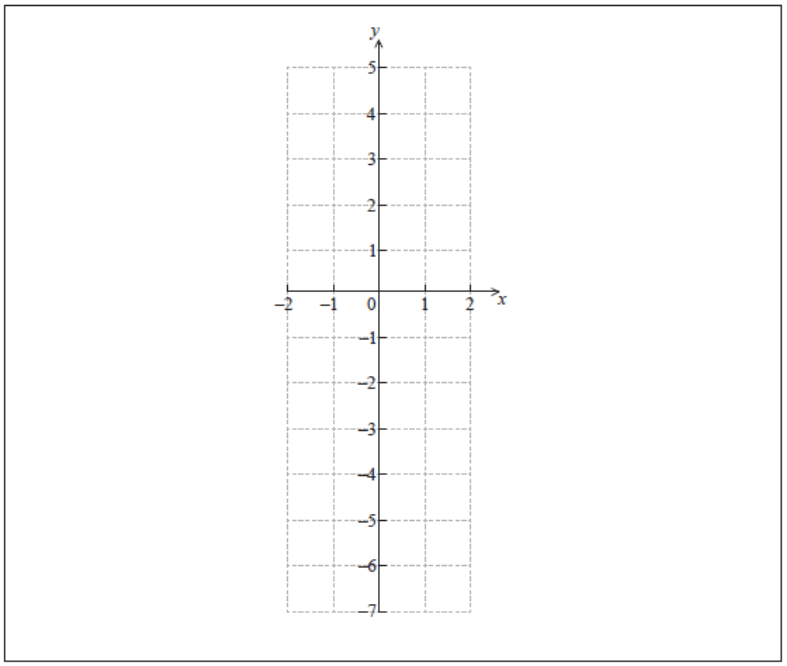
\includegraphics[scale=0.3]{grid_5_12}\par
  \end{flushleft}
\end{question}


